\documentclass[spanish,12pt,letterpaper]{article}

\usepackage[spanish]{babel}
\usepackage[utf8x]{inputenc}
\usepackage{authblk}
\usepackage{listings}
\usepackage{dsfont}
\usepackage{graphicx}
\usepackage{enumerate}
\usepackage{float}
\usepackage{amsmath}
\usepackage{pgfplots}
\usepackage{pst-plot}
\usepackage{pstricks}
\usepackage{scrextend} %Ref to previous footnote
\usepackage[ruled,vlined, linesnumbered]{algorithm2e}
\usepackage{tikz}
\usetikzlibrary{trees,arrows,positioning, calc}
\tikzstyle{redVertex}  =[draw,fill=red,     circle,minimum size=18pt,inner sep=0pt, text=white]
\tikzstyle{blackVertex}=[draw,fill=black,   circle,minimum size=18pt,inner sep=0pt, text=white]
\tikzstyle{nil}        =[draw,fill=black,rectangle,minimum size=5pt,inner sep=0pt, text=white]

\newcommand{\QED}{\hfill \textit{\textbf{Q.E.D.}}}

\title{Tarea 01 Estructuras de Datos Avanzadas}
\author{Emiliano Galeana Araujo}
\affil{Facultad de Ciencias, UNAM}
\date{\today}

\begin{document}

\maketitle

\begin{enumerate}
\item Demostrar que dados dos árboles binarios ordenados de búsqueda \textit{T} y
  \textit{T'} con $n$ nodos, podemos convertir a \textit{T} en \textit{T'}
  haciendo $O(n)$ rotaciones. Hint: Demostrar que cualquier árbol puede ser
  transformado en uno fijo (Un camino por ejemplo) con $O(n)$ rotaciones.\\
  Consideremos la transformación de un árbol binario ordenado de búsqueda
  \textit{T} en una 'cadena' hacia la derecha como sigue. Dejamos a la raíz y a
  los elementos que son hijos derechos como elementos de la 'cadena derecha'.
  Para cualquier nodo que sea hijo izquierdo, podemos agregar este nodo a la
  'cadena derecha' haciendo una rotación a la derecha sobre su padre. Entonces,
  podemos convertir cualquier árbol binario de búsqueda \textit{T} en una 'cadena
  derecha' con a lo más $n-1$ rotaciones $\in O(n)$.\\
  Sea $(r_1, r_2, ..., r_k)$ la secuencia de rotaciones para convertir \textit{T} 
  en una 'cadena derecha' y sea $(s_1, s_2, ..., s_m)$ la secuencia de rotaciones 
  para convertir otro árbol binario de búsqueda \textit{T'} en una 'cadena
  derecha', entonces $k < n, m < n$ siendo $n$ el número de elementos en el
  árbol. Y así podemos convertir a \textit{T} en \textit{T'} con la siguiente
  secuencia $(r_1, r_2, ..., r_k, s'_1, s'_2, ..., s'_m)$ donde $s'_i$ es la
  rotación contraria de $s_i$.\\
  Como $k+m < 2n$, el número de rotaciones necesarias es $O(n)$.
  
\item Una familia de árboles es balanceada, si todo árbol de la familia tiene
  altura $O(log(n))$, donde $n$ es el número de nodos en el árbol. Determina si
  las siguientes familias de árboles binarios, son familias balanceadas.
  Justifica tu respuesta.
  \begin{enumerate}[a)]
  \item Todo nodo del árbol es una hoja o tiene dos hijos.\\
    Contraejemplo, consideremos el siguiente árbol:\\
    \begin{center}
    \begin{tikzpicture}[font=\sffamily,scale=0.6,very thick,level/.style={sibling distance=80mm/#1}]
      \node [blackVertex] (r){.}
      child {
        node [blackVertex] {.}
      }
      child {
        node [blackVertex] {.}
        child {
          node [blackVertex] {.}
        }
        child {
          node [blackVertex] {.}
          child {
            node [blackVertex] {.}
          }
          child {
            child {
              node [blackVertex] {.}
              child {
                node [blackVertex] {.}
              }
              child {
                child {
                  node [blackVertex] {.}
                  child {
                    node [blackVertex] {.}
                  }
                  child {
                    node [blackVertex] {.}
                  }
                }
              }
            }
          }
        }
      };
    \end{tikzpicture}
    \end{center}
    Podemos ver que todo árbol generado cone ssas condiciones tienen exactamente
    dos nodos en cada nivel (Exceptuando la raíz) y por la definición dada, no
    tiene altura $O(log(n))$. Es un caso particular de la familia, pero ya no
    cumple ser balanceado.
  \item Existe una constante $c$ tal que, para cada nodo en el árbol, las alturas
    de sus subárboles difieren a lo más $c$.\\
    Prueba basada en la demostración de que los árboles \textit{AVL} tienen
    altura logarítmica\footnote{https://cs.nyu.edu/courses/fall02/V22.0310-002/
      lectures/lecture-16.html}.\\
    Sea \textit{T} un árbol que cumpla la propiedad $b$, queremos ver que $T$ con
    altura $h$ tiene al menos $2^{\frac{h}{2+c}-1}$ nodos internos.\\
    Sea $n(h)$ el mínimo número de nodos internos en T...\\
    n(1) = 1 y n(2) = 2.\\
    Cuando n $\geq$ 3
    \[n(h) = 1 + n(h-1) + n(h-1-c)\]
    \[n(h) = 1 + 1 + n(h-2) + n(h-2-c) + 1 + n(h-2-c) + n(h-2-2c)\]
    \[n(h > 2n(h-2-c))\]
    Aplicando esto $i$ veces, tenemos
    \[i > 0, n(h) > 2^{\frac{h}{2+c}-1}\]
    Entonces, un árbol que cumple $b$, tiene $2^{\frac{h}{2+c}-1}$ nodos internos.
    Falta ver ue la altura es logarítmica.\\
    De lo anterior, tenemos.
    \[n(h) > 2^{\frac{h}{2+c}-1}\]
    \[log(n(h)) > \frac{h}{2+c}-1\]
    \[log(n(h))-1 > \frac{h}{2+c}\]
    \[(2+c)log(n(h))-1 > h\]
    Entonces podemos ver que los árboles que cumplen $b$, tienen altura
    logarítmica y por lo tanto son balanceados.
  \end{enumerate}
  
\item Considera el treap \textit{T} después de insertar $x$, con el algoritmo
  visto en clase. Sea $C$ la longitud del camino derecho del subárbol izquierdo
  de $x$. Sea $D$ la longitud del camino izquierdo del subárbol derecho de $x$.
  Demuestre que el número total de rotaciones que se realizaron durante la
  inserción de $x$ es igual a $C + D$.\\
  Base. Cuando $x$ después de insertar, termina como hoja. Entonces $C = 0,
  D = 0$.
  Hipótesis. Insertamos $x$ y no termina como hoja, entonces $C = n, D = m$, y se
  necesitaron $C+D = n+m$ rotaciones para llevar a $x$ a su lugar.
  Paso inductivo. En la inserción de $x$, $x.key < x.padre.key$, eso quiere decir
  que hace falta una rotación para subir a $x$ a su lugar. Por hipotesis, tenemos
  que $C = n, D = m$, hacemos la rotación sin pérdida de generalidad y ahora $x$
  está en su lugar, pues todas las llaves en el treap son menores o iguales a
  $x.key$, entonces, aumentamos en 1 el camino de $C$ o $D$, (Pues cada vez que
  hacemos un giro, la altura del subárbol contrario al giro cambia en 1 ).
  Entonces $C = n+1, D = m$ por lo tanto los cambios necesarios para insertar
  correctamente a $x$ fueron $C+D$.
  
\item Describe una secuencia de accesos a un árbol splay \textit{T} de $n$ nodos,
  con $n > 5$ impar, que resulte en \textit{T} siendo una sola cadena de nodos en
  la que el camino para bajar en el árbol alterne entre hijo izquierdo e hijo
  derecho.\\
  Para lograrlo, hay que colocar al nodo con el mayor elemento en la raíz, y como
  hijo al nodo con menor elemento como su hijo, y así sucesivamente. Por lo que
  el nodo con el nodo mayor tiene que ser el último accesado y el nodo con menor
  elemento el penúltimo. La secuencia de accesos la podemos ver en dos partes:
  \begin{itemize}
  \item Primero necesitamos llevar nuestro árbol splay a un camino descendente,
    esto se puede lograr accediendo a los n elementos del árbol en órden
    ascendente ($1,2, ..., n$).
  \item Luego, basta calcular la siguiente serie, que termina cuando intentemos
    acceder al elemento máximo $(n)+1$. NOTA: en la división, se toma el piso.
    \begin{align*}
      \frac{n}{2}, \frac{n}{2}+2, \frac{n}{2}+3, \frac{n}{2}+2, \frac{n}{2}-1,
      \frac{n}{2}+3, \frac{n}{2}+4, \frac{n}{2}+3, \frac{n}{2}-2, \frac{n}{2}+4,
      \\
      \frac{n}{2}+5, \frac{n}{2}+4, \frac{n}{2}-3, ... \frac{n}{2}+k = n+1
    \end{align*}
  \end{itemize}
  ¿Por qué tiene que ser mayor a 5? Porque si n = 3 $\frac{n}{2}+2$ = 4 y ese
  elemento no existe, y nos regresa el mismo árbol secuencial con la raíz el
  mayor elemento.\\
  
\item Demuestre o da un contraejemplo:
  \begin{enumerate}[a)]
  \item Los nodos de cualquier árbol \textit{AVL} pueden colorearse de rojo y
    negro para obtener un árbol rojo-negro válido.\\
    Podemos colorear los nodos de nuestro árbol \textit{AVL} de rojo si cumplen:
    \begin{itemize}
    \item No ser la raíz.
    \item Si su altura es par.
    \end{itemize}
    De cualquier otra forma, coloreamos los nodos de color negro.\\
    Tenemos que ver que con estas condiciones se satisfagan las siguientes
    propiedades:
    \begin{itemize}
    \item Todos los nodos son rojos o negros.
    \item Las hojas $null$  y la raíz son negras.
    \item Si un nodo es rojo, sus hijos son negros.
    \item Todos los caminos de un nodo a alguna de sus hojas tienen el mismo
      número de nodos negros.
    \end{itemize}
    Dadas nuestras condiciones, tenemos que todos los nodos tienen un color.
    También que la raíz y las hojas null son negras. Por que coloreamos de rojo a
    los nodos con altura par y de negro si son impares, entonces no hay un nodo
    rojo con hijos rojos. Falta ver que cualquier camino de un nodo a sus hijos
    tiene el mismo número de nodos negros.\\
    Sabemos que al ser un árbol \textit{AVL}, entonces tiene la mayoría de sus
    niveles completos, entonces podemos afirmar que hasta el último nivel que se
    encuentre completo se cumple la propiedad, pues solo es un caso particular de
    un árbol \textit{rojo-negro}, el caso donde cada nivel tiene un color
    distinto. ¿Qué pasa si el último nivel no está completo? Pues todas las hojas
    son de color negro, pues no tienen algura par (por nuestras condiciones), así
    para cualquier nodo interno los caminos a sus hojas se van alternando en
    color, entonces cualquier camino de un nodo a sus hijos tiene el mismo número
    de nodos negros.
  \item Cualquier árbol rojo-negro satisface las propiedades de árbol
    \textit{AVL}.\\
    Contraejemplo, el siguiente árbol no cumple las propiedades de \textit{AVL},
    pues podemos notar que la altura de los subárboles del nodo 5, difieren en
    más de 1.\\ 
    
    \begin{tikzpicture}[font=\sffamily,very thick,level/.style={sibling distance=80mm/#1}]
      \node [blackVertex] (r){5}
      child {
        node [blackVertex] {2}
        child {node [nil] {NIL}}
        child {node [nil] {NIL}}
      }
      child {
        node [redVertex] {7}
        child {
          node [blackVertex] {5}
          child {node [nil] {NIL}}
          child {node [nil] {NIL}}
        }
        child {
          node [blackVertex] {10}
          child {
            node [redVertex] {8}
            child {node [nil] {NIL}}
            child {node [nil] {NIL}}
          }
          child {
            node [redVertex] {13}
            child {node [nil] {NIL}}
            child {node [nil] {NIL}}
          }
        }
      };
    \end{tikzpicture}
  \end{enumerate}
  
\item Modifica el árbol splay para que pueda hacer consultas del $k$-ésimo
  elemento más chico.\\
  Podemos modificar los nodos para que tengan una variable que guarde el número
  de nodos totales en el subárbol. Por ejemplo, la raíz tiene en esa variable, el
  número total de elementos en el árbol, y ese número se calcula sumando las
  varibles de su hijo izquierdo y derecho (En caso de que no tenga alguno, no
  importa, pues sería 0). ¿Cómo acceder al $k$-ésimo elemento más chico? El
  siguiente algoritmo lo muestra.
  \begin{center}
    \begin{algorithm}[H]
        \SetKwInOut{Input}{inputs}
        \SetKwInOut{Output}{output}
        \SetKwProg{getKthElement}{getKthElement}{}{}
        
        \getKthElement{k int, root node}{
          \Input{k un entero positivo, el nodo raíz de un árbol Splay del que
            queremos el $k$-ésimo elemento}
          \Output{node(e) con e el $k$-ésimo elemento más chico}
          \State $i \gets 0$\\
          \If{root.left != null}{
            \State $i \gets root.left.elementos$
          }
          \If{$k < i$}{
            \KwRet{getKthElement(k, root.left)}
          }\ElseIf{$k == i$}{
            \KwRet{root}
          }\Else{
            \KwRet{getKthElement(k-1-i, root.right)}
          }
          \EndIf
        }
        \caption{Get k-th element}
    \end{algorithm}
\end{center}


  
  
\item Explica cómo obtener el mínimo valor almacenado en un árbol $B$ y cómo
  encontrar al predecesor de un valor almacenado $x$ en un árbol $B$.\\
  \begin{itemize}
  \item mínimo: Basta ir al hijo más pequeño recursivamente hasta encontrar que
    no tiene hijos, o sea, es null, y entonces tomar el primer valor del nodo.
  \item predecesor: Para encontrar al predecesor de $x$, primero encontramos a
    $x$ partiendo de la raíz del árbol. Una vez encontrado tenemos dos casos.
    \begin{itemize}
    \item Si el elemento tiene hijo izquierdo, entonces tenemos que encontrar
      al elemento más grande en el subárbol izquierdo. Que es movernos al hijo
      izquierdo y mientras su hijo derecho sea distinto de null, seguimos
      avanzando.
    \item Si el elemento no tiene hijo izquierdo, entonces tenemos que subir un
      nivel (Al padre del elemento.)
    \end{itemize}
  \end{itemize}
  
\item ¿Cuál es el número esperado exacto de nodos en una skip list que almacena
  $n$ valores? no cuentes el súper inicio y el súper final.\\
  %% https://nscpolteksby.ac.id/ebook/files/Ebook/Computer%20Engineering/Open%20Data%20Structures%20(2013)/Chapter%204%20-%20Skiplists.pdf
  %% http://opendatastructures.org/ods-cpp/4_4_Analysis_Skiplists.html#tex2html39
  Recordemos que una skiplist es una secuencia de listas simplemente ligadas
  $(l_0, l_1, ..., l_h)$ en donde cada $l_r$ contiene un subconjunto de elementos
  en $l_{r-1}$ (La lista completa es $l_0$).\\
  $2n$. La probabilidad de que cualquier elemento 'x' esté en la lista $l_r$ es
  $\frac{1}{2^r}$, entonces el número esperado de elementos en $l_r$ es
  $\frac{n}{2^r}$. Entonces el número total de nodos esperados en todas las
  listas es:
  \[\sum_{r=0}^{\infty} \frac{n}{2^r} = n(1 + \frac{1}{2} + \frac{1}{4} +
  \frac{1}{8} + ...) = 2n\]
  
\item Describe cómo modificar una skip list $L$ para poder realizar las
  siguientes dos operaciones en tiempo esperado $O(logn)$.\\
  Podemos modicar las skip-list con algo conocido como \textit{width of the link}
  \footnote{https://en.wikipedia.org/wiki/Skip\_list#Indexable\_skiplist
  \label{skiplist}}
  que lo que hace es guardar en los enlaces de los nodos el peso de estos. El
  peso del enlace en $l_i$ se define como el número de enlaces que se salta en
  $l_{i-1}$. En la siguiente figura\footref{skiplist} podemos ver una skip-list
  con \textit{width of the link}.
  \begin{center}
    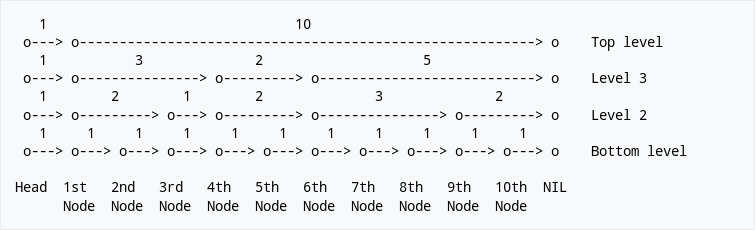
\includegraphics[scale=.5]{../imagenes/skiplist.jpg}
  \end{center}
  \begin{enumerate}[a)]
  \item Dado un índice $i$, obtener el elemento de $L$ en la posición $i$.\\
    Si queremos encontrar el $i$-ésimo elemento, basta empezar por el primer
    nivel y pasarnos al siguiente (más alto) le preguntamos a nuestro enlace qué
    valor tiene. Si es mayor a $i$, entonces nos pasamos de $i$, así que no
    avanzamos y tenemos que bajar un nivel desde el nodo actual. Si es menor,
    entonces nos pasamos al nodo que nos lleva ese enlace y restamos a $i$ el
    valor del enlace. Terminamos cuando $i$ sea igua a $0$.
  \item Dado un valor $x$, obtener la cantidad de elementos en $L$ menores a $x$.
    \\
    Tenemos que pararnos en el primer nivel y avanzar al siguiente, si es mayor a
    $x$, entonces nos pasamos del objetivo, así que no avanzamos  y descendemos
    un nivel en el nodo actual. Si es menor a $x$, guardamos el valor del enlace
    y seguimos buscando hacia adelante. Finalmente, si el siguiente nodo es $x$,
    entonces regresamos la suma acumulada.
  \end{enumerate}
\item Sea $P$ un conjunto de $n$ puntos en el plano. La escalera de $P$ es el
  conjunto de todos los puntos en el plano que tienen al menos un punto en $P$
  tanto arriba como a la derecha.
  \begin{itemize}
  \item Describir un algoritmo para calcular la escalera del conjunto de $n$
    puntos en tiempo $O(nlogn)$.\\
    Usando la estructura descrita abajo, podemos ir agregando los puntos en orden
    para al final tener en la raíz a los máximos del conjunto. Recorrer los
    puntos nos toma $O(n)$, y ordenar los puntos para recorrerlos $O(nlogn)$,
    agregar a la estructura $O(log²n)$, entonces podemos calcular la escalera de
    $P$ en $O(nlogn)$.
  \item Describir y analizar una estructura de datosque guarde la escalera del
    conjunto de puntos y un algoritmo \texttt{ABOVE? (x,y)} que regrese \texttt{
      TRUE} si el punto \texttt{(x,y)} está por encima de la escalera, o \texttt{
      FALSE} en otro caso. La estructura de datos tiene que usar $O(n)$ en
    espacio, y el algoritmo \texttt{ABOVE?} tique que ejecutarse en tiempo
    $O(nlogn)$.\\
    Podemos usar una estructura de datos parecida a \footnote{``M.H. Overmars and
      J. Van Leeuwen, Maintenance of Configurations in the Plane, 1981.''} la
    cual toma $O(n)$ en espacio y puede ser creada en $O(nlogn)$. Y funciona como
    sigue.\\
    En cualquier momento el conjunto de máximos de $P$ se encuentra en la raíz,
    en una cola concatenable.
    Definimos a los máximos de $P$ como: el conjunto de elementos máximos de $P$.
    Decimos que un elemento es máximo si ningún otro punto lo domina. Decimos que
    un punto $x$ domina a otro $y$ si $x \in Dom(y)$ y. Definimos al conjunto
    $Dom(y)$ como los puntos que están a la izquierda y por debajo de $y$.
    Entonces un punto $x$ domina a $y$ syss $X(x) > X(y)$ y también $Y(x) > Y(y)$
    . Y pues ya, la raiz que contiene a los máximos de $P$ es nuestra escalera.\\
    Nuestro algoritmo \texttt{ABOVE?} funciona tomando al punto $(x,y)$ y lo
    insertamosa la raíz de nuestra estructura, lo que va a hacer es encontrar a
    $Y(x)$, y partir la estructura en dos ($T_{down}, T_{up}$), en donde $T_{down}$
    contiene al los máximos del domino de $(x,y)$ el punto a insertar. Si es
    vacío, entonces $(x,y)$ está dentro de la escalera, sino, está afuera.
  \end{itemize}
\end{enumerate}

\end{document}
